\section{Introduction}

\begin{frame}
    \frametitle{The Clean Energy Transition}
    Our changing climate and additional demand drivers from data 
    centers and \gls{ai} require a just transition from fossil 
    fuels to clean energy.
\end{frame}

\begin{frame}
    \frametitle{Three tenets of justice}
    \begin{figure}
        \centering
        % \resizebox{0.7\columnwidth}{!}{
            \begin{tikzpicture}
                \begin{scope}[blend group = soft light]
                    % \fill[red!30!white]   ( 90:1.2) circle (2);
                    \fill[illiniorange]   ( 90:1.2) circle (2);
                    % \fill[green!30!white] (210:1.2) circle (2);
                    \fill[illiniorange] (210:1.2) circle (2);
                    % \fill[blue!30!white]  (330:1.2) circle (2);
                    \fill[illiniorange]  (330:1.2) circle (2);
                \end{scope}
                \node at ( 90:2)    {Recognition}; 
                \node at ( 210:2) {Distribution}; 
                \node at ( 330:2)   {Procedural}; 
                \node[font=\Large] {\textcolor{black}{Justice}};
              \end{tikzpicture}

        % }
        \caption{Three aspects of justice \cite{schlosberg_1_2007}.}
    \end{figure}
\end{frame}

\begin{frame}
    \frametitle{\glspl{esom}}
    \Glspl{esom} are a class of tools designed to 
    optimize this transition. (Provide examples?)

    They will become more important with more \gls{vre}
    and more volatile weather.

    \textit{But they have at least two big flaws}.
    \begin{enumerate}
        \item All current \glspl{esom} optimize a single objective --- cost.
        \item \glspl{esom} struggle to model the ``human dimension'' thereby
        limiting their ability to address justice \cite{pfenninger_energy_2014}.

    \end{enumerate}
\end{frame}

\begin{frame}
    \frametitle{\gls{osier}}
    I developed \gls{osier} to fill these gaps by \cite{dotson_osier_2024}
    \begin{enumerate}
        \item optimizing multi- and many-objective problems,
        \item allowing user-defined objectives.
    \end{enumerate}
    [Show the 4-objective problem from the prelim]
\end{frame}

\begin{frame}
    \frametitle{How \gls{osier} Works}

    \begin{figure}
        \centering
        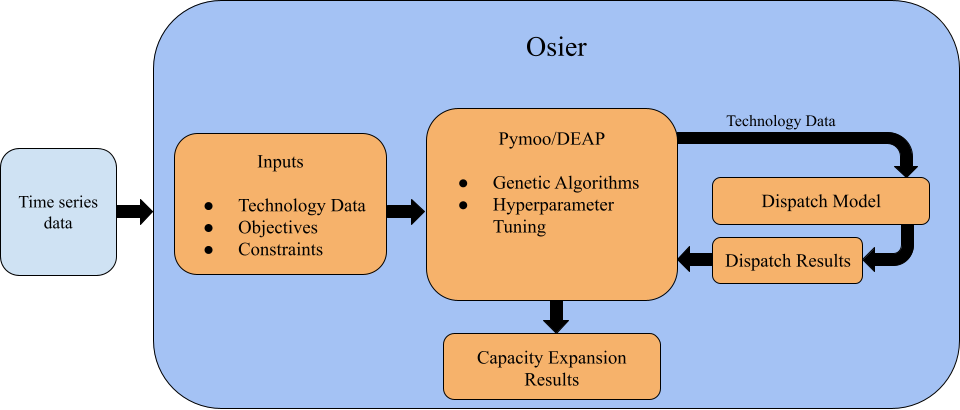
\includegraphics[width=\columnwidth]{../docs/figures/03_osier_chapter/osier_flow.png}
        \caption{Flow of data into and within \gls{osier}}
        \label{fig:osier-flow}
    \end{figure}
    % [Show the data flow diagram]

    % Osier works by leveraging genetic algorithsm... 
\end{frame}

\begin{frame}
    \frametitle{Goals from Preliminary Exam}

    The goals fall into two large buckets

    \begin{enumerate}
        \item \boldorange{Improve} \gls{osier} by
        \begin{enumerate}
            \item Adding a new, faster, dispatch algorithm
            \item Developing an enhanced \gls{mga} algorithm
        \end{enumerate}
        \item \boldorange{Validate} \gls{osier}'s usefulness through a 
        multiple-case study of energy decision-making in Illinois.
    \end{enumerate}
\end{frame}

\begin{frame}
    \frametitle{Objectives of this presentation}
    \begin{enumerate}
        \item Show the technical improvements to \gls{osier}.
        \item Demonstrate how \gls{osier} can be used to evaluate nuclear fuel cycle options.
        \item Share the results from the case study.
    \end{enumerate}
\end{frame}